\section{Vorkommen und Vermeidbarkeit}
\subsection{Vorkommen und Verwendungszweck}
Bisphenol-A ist eine im Alltag sehr schwer zu vermeidbare Chemikalie, wie schwer
wird einem jedoch erst klar wenn man sieht in welchen Produkten es steckt.
Kunststoffe, besonders die aus Epoxidharz und Polycarbonat
beinhalten Bisphenol-A. Polycarbonate sind thermoplastische Kunststoffe
und besitzen eine sehr hohe Festigkeit, Steifheit, Härte und Schlagzähigkeit \cite{Umweltbundesamt2010}.
Sie sind außerdem hervorragende Isolatoren gegen elektrische Spannung.
Sie zeigen eine hohe Beständigkeit gegenüber Wasser, Öle und Fette, sowie
Strahlungseinflüsse. Polycarbonate sind entflammbar(erlischt jedoch nach entfernen der Zündquelle) \cite{Umweltbundesamt2010} und erfüllen die Anforderungen
der Brandklasse B2 \cite{Wikipedia}.
\begin{figure}[htpb]
    \centering
    \includegraphics[width=.75\textwidth]{Plastikgeschirr.jpeg}
    \caption{Plastikgeschirr \cite{Plastikgeschirr}}
\end{figure}
Aus diesem Kunststoff, werden zum Beispiel Artikel wie Plastikgeschirr
hergestellt, welche einen direkten Kontakt mit
Nahrungsmitteln bieten. Aber auch sicherheitstechnisch wichtige Dinge wie
Motorradhelme bestehen aus Polycarbonaten. Außerdem sollte der
medizinische Bereich nicht vergessen werden, bei der zum Beispiel
Geräte zur Analyse aus Polycarbonaten bestehen, sowie einige Werkzeuge
\cite{Umweltbundesamt2010}.
\begin{figure}[htpb]
    \centering
    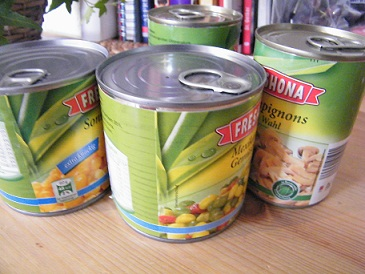
\includegraphics[width=.5\textwidth]{Konserven.jpg}
    \caption{Konservendosen \cite{Konserven}}
    \end{figure}
Epoxidharze sind Kunstharze, welche sich zunächst im flüssigen Zustand befinden
und mit einem Härter $($Reaktionspartner$)$ zu duroplastischen Kunststoffen
umgesetzt werden\cite{Umweltbundesamt2016}. \glqq Die durch Vernetzung erzeugten
Duroplaste besitzen gute mechanische Eigenschaften sowie eine gute Temperatur-
und Chemikalienbeständigkeit\grqq{\cite{Epoxidharz}}. Epoxidharze sind
hochwertige, jedoch teure Kunststoffe. Epoxidharze werden größtenteils \glqq als
Kleb-,Lack- und Gießharze für Oberflächenbeschichtungen genutzt\grqq{}{\cite{Umweltbundesamt2016}}.
Getränke-/Konserven-Dosen können zum Beispiel innen mit Epoxidlack beschichtet sein \cite{Bund}.
\subsection{Vermeidbarkeit}
Bisphenol-A komplett zu meiden erweist sich in unserer heutigen
fortgeschrittenen Gesellschaft vor allem aus medizinischer
Sicht als sehr schwer, trotzdessen ist es gut möglich auf einige Bisphenol-A haltige Produkte zu verzichten bzw. einen Ersatz zu finden.\\
Hier einige Beispiele von \cite{Utopia}:
\begin{itemize}
    \item Lebensmittel in Kunststoffbehältern nicht erhitzen, da sonst dadurch Bisphenol A freigesetzt werden kann.
    \item Lebensmittel allgemein in Behältern bestenfalls aus Glas, Keramik oder Edelstahl lagern.
    \item Beim Kauf kunststoffhaltiger Produkte auf den Hinweis \glqq BPA free\grqq{} achten.
    \item Polycarbonat-Produkte meiden $($wird mit dem Recyclingcode RE 7 abgekürzt$)$.
    \item Als Trinkflasche eine aus Glas oder unbeschichtetem Edelstahl.
\end{itemize}
Ein weiterer nennenswerter positiver Effekt, wenn man oben genannte Behältern
und Trinkflaschen nutzt, ist die hervorragend funktionierende Wiederverwendbarkeit
der Produkte. Und das Wiederverwenden wirkt
unserer \glqq Wegwerfgesellschaft\grqq{} entgegen, weshalb man damit auch der Umwelt
positiv entgegen kommt und für mehr Nachhaltigkeit sorgt.
